\documentclass[12pt]{article}

% Essential packages for mathematics
\usepackage{amsmath}    % Advanced math environments
\usepackage{amssymb}    % Additional math symbols
\usepackage{amsthm}     % Theorem environments
\usepackage{mathtools}  % Extensions to amsmath

% Algorithm packages
\usepackage[ruled,vlined]{algorithm2e}  % Popular algorithm package
% Alternative: \usepackage{algorithm,algpseudocode} % For algorithmicx

% Other useful packages
\usepackage{graphicx}   % For including figures
\usepackage{geometry}   % Page layout
\usepackage{hyperref}   % Hyperlinks
\usepackage{cleveref}   % Smart cross-referencing
\usepackage{dirtree}
\usepackage{float} 
% Page setup
\geometry{margin=1in}
\setlength{\parindent}{0pt}
\setlength{\parskip}{1em}

% Theorem environments
\newtheorem{theorem}{Theorem}[section]
\newtheorem{lemma}[theorem]{Lemma}
\newtheorem{corollary}[theorem]{Corollary}
\newtheorem{proposition}[theorem]{Proposition}
\theoremstyle{definition}
\newtheorem{definition}[theorem]{Definition}
\newtheorem{example}[theorem]{Example}
\theoremstyle{remark}
\newtheorem{remark}[theorem]{Remark}

% Custom math operators
\DeclareMathOperator{\argmax}{arg\,max}
\DeclareMathOperator{\argmin}{arg\,min}
\DeclareMathOperator{\E}{\mathbb{E}}
\DeclareMathOperator{\Var}{Var}
\DeclareMathOperator{\Cov}{Cov}

% Algorithm2e settings
\SetAlgoNlRelativeSize{0}  % Line numbers same size as text
\SetAlgoNoLine             % Remove vertical lines (comment to keep them)
\DontPrintSemicolon        % Don't print semicolons at end of lines

\title{Discussion on Project}
\author{Harshit Rawat}
\date{\today}

\begin{document}

\maketitle
\section{Preliminary observations}
Our project can be understood with the following structure:
\medskip
\dirtree{%
.1 Molecule name 5(aspirin trained using 5 examples).
.2 random\_seed\_42.
.3 lr\_10(Ensemble).
.4 model\_1.
.4 model\_2.
.4 model\_3.
.4 model\_4.
.4 model\_5.
.3 lr\_20.
.4 model\_1.
.4 model\_2.
.4 \ldots .
.2 random\_seed\_52.
.1 Molecule name 10(aspirin trained using 10 examples).
}


\newpage
\section{Preliminary Model Selection Framework and Results}
\begin{algorithm}[htbp]
\caption{Median Based Algorithm for Model Selection}\label{alg:Median algorithm}
\KwIn{Set of ensembles $\mathcal{E}$, each ensemble contains 5 models}
\KwOut{Best Ensemble}

\ForEach{ensemble $E \in \mathcal{E}$}{
    \ForEach{model $m \in E$}{
        Evaluate $m$ \textbf{energy\_mae} of model on it's   \textbf{personal} validation set\;
        This will be used as \textbf{model performance metric}. \;
    }
    Compute median of performance of models in $E$\;
}
Select ensemble with best median performance\;
\end{algorithm}
\begin{table}[htbp]
\centering
\small
\caption{Energy and Force MAE (mean $\pm$ std) for different numbers of examples.}
\begin{tabular}{@{}lcccc@{}}
\hline
\textbf{num\_ex} & \textbf{NEAL Energy} & \textbf{Vanilla Energy} & \textbf{NEAL Force} & \textbf{Vanilla Force} \\
& \textbf{MAE} & \textbf{MAE} & \textbf{MAE} & \textbf{MAE} \\
\hline
5  & 343.26 $\pm$ 100.34 & \textbf{288.08 $\pm$ 51.77}  & 364.96 $\pm$ 93.60  & \textbf{313.23 $\pm$ 22.08} \\
10 & 205.71 $\pm$ 23.73  & \textbf{203.09 $\pm$ 32.34}  & \textbf{242.51 $\pm$ 20.24}  & 247.44 $\pm$ 27.42 \\
20 & \textbf{108.13 $\pm$ 15.15}  & 131.57 $\pm$ 7.77   & 175.42 $\pm$ 4.13   & \textbf{173.97 $\pm$ 4.24}  \\
40 & \textbf{75.56  $\pm$ 5.01}   & 87.26  $\pm$ 16.59  & 142.85 $\pm$ 7.09   & \textbf{138.52 $\pm$ 2.94}  \\
\hline
\end{tabular}
\\[5pt] % This adds a vertical space of 5 points after the table.
Note: Values slightly different from the ones reported in ppt as I directly took avg in pandas.
\end{table}
\begin{figure}[H]
    \centering
    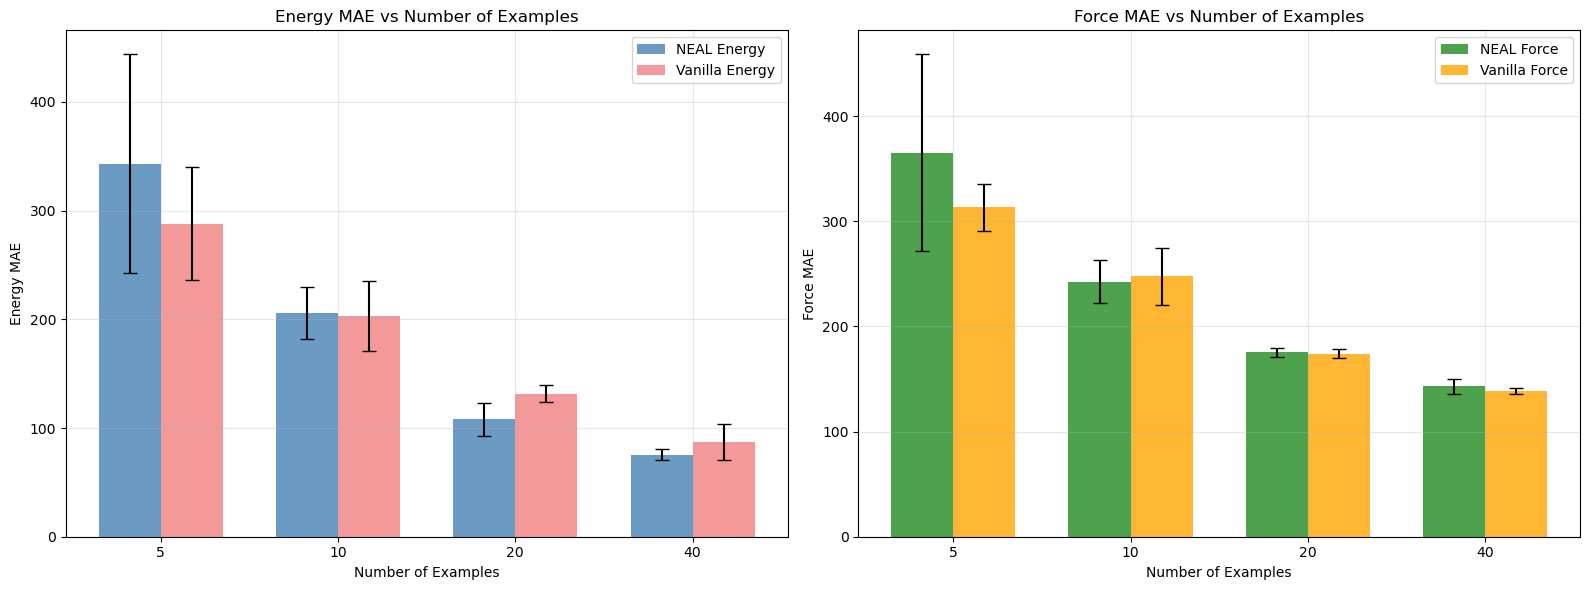
\includegraphics[width=1.0\linewidth]{plots/plots_for_median_strategy_using_only_train_energy.png}
    \caption{Median strategy for combination using energy mae as perf measure.}
    \label{fig:placeholder}
\end{figure}
\newpage
\section{Model Selection via Validation Set of 500 unseen examples}
Each ensemble was evaluated on the validation set and the model with lowest validation loss was selected for each seed. To ensure a fair comparison \textbf{vanilla} models were also evaluated across their hyperparameters on validation set.
\begin{table}[htbp]
\centering
\small
\caption{Energy and Force MAE (mean $\pm$ std) for different numbers of examples.}
\begin{tabular}{@{}lcccc@{}}
\hline
\textbf{num\_ex} & \textbf{NEAL Energy} & \textbf{Vanilla Energy} & \textbf{NEAL Force} & \textbf{Vanilla Force} \\
& \textbf{MAE} & \textbf{MAE} & \textbf{MAE} & \textbf{MAE} \\
\hline
5  & \textbf{243.72 $\pm$ 41.24} & 254.80 $\pm$ 39.75  & \textbf{281.81 $\pm$ 14.55} & 289.37 $\pm$ 16.08 \\
10 & \textbf{166.55 $\pm$ 29.73} & 178.93 $\pm$ 20.54  & 232.83 $\pm$ 19.25 & \textbf{232.06 $\pm$ 14.46} \\
20 & \textbf{99.75 $\pm$ 11.23}  & 131.58 $\pm$ 7.78   & 177.79 $\pm$ 2.83  & \textbf{173.97 $\pm$ 4.24} \\
40 & \textbf{69.80 $\pm$ 3.80}   & 87.27 $\pm$ 16.58   & 140.74 $\pm$ 6.37  & \textbf{138.52 $\pm$ 2.94} \\
\hline
\end{tabular}
\end{table}
\begin{figure}[htbp]
    \centering
    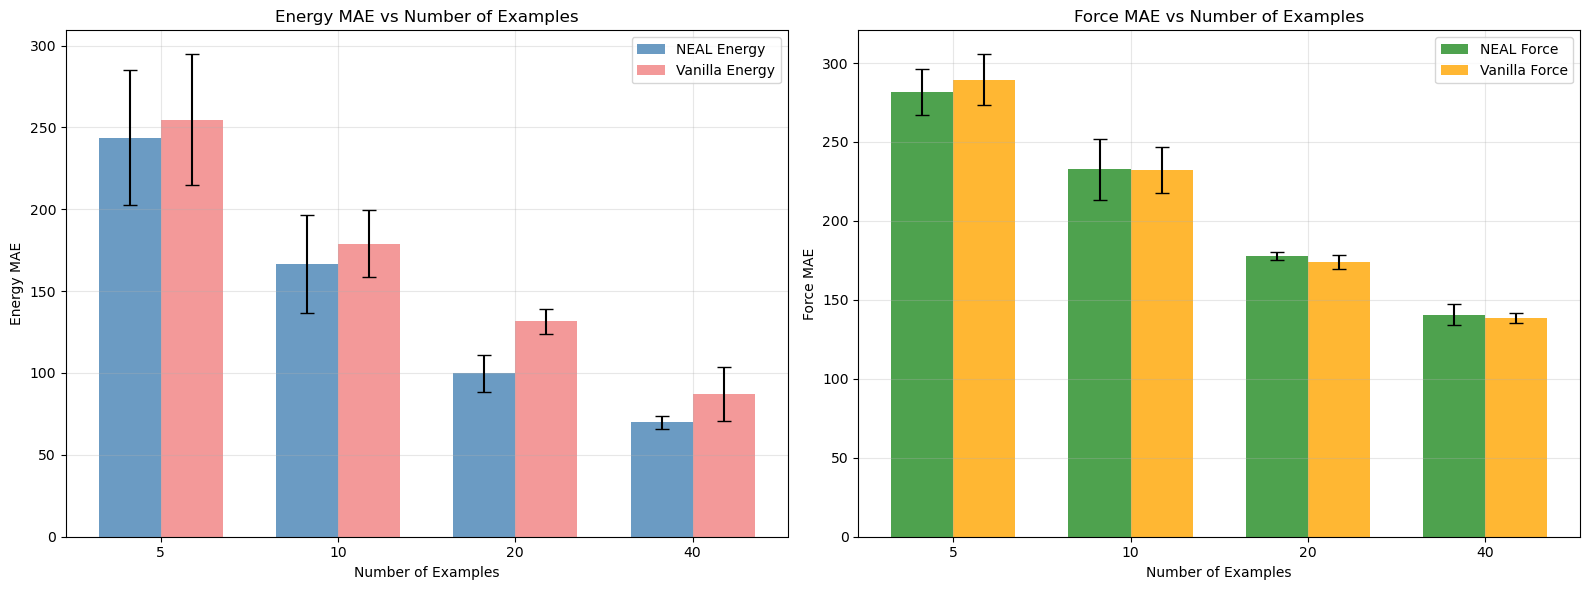
\includegraphics[width=1.0\linewidth]{plots/validation on 500 examples using enerhy mae.png}
    \caption{Using energy mae with a validation set of 500 examples.}
    \label{fig:placeholder}
\end{figure}

Repeating the experiments using only force\_mae.
\begin{table}[htbp]
\centering
\small
\caption{Energy and Force MAE (mean $\pm$ std) for different numbers of examples.}
\begin{tabular}{@{}lcccc@{}}
\hline
\textbf{num\_ex} & \textbf{NEAL Energy} & \textbf{Vanilla Energy} & \textbf{NEAL Force} & \textbf{Vanilla Force} \\
& \textbf{MAE} & \textbf{MAE} & \textbf{MAE} & \textbf{MAE} \\
\hline
5  & \textbf{252.82 $\pm$ 41.68} & 254.81 $\pm$ 39.76 & \textbf{280.94 $\pm$ 14.57} & 289.37 $\pm$ 16.08 \\
10 & \textbf{173.87 $\pm$ 34.88} & 180.64 $\pm$ 20.52 & \textbf{221.50 $\pm$ 10.83} & 225.99 $\pm$ 6.40 \\
20 & \textbf{122.49 $\pm$ 17.06} & 131.60 $\pm$ 7.77  & \textbf{172.41 $\pm$ 3.43}  & 173.97 $\pm$ 4.24 \\
40 & \textbf{81.05 $\pm$ 14.19}  & 87.26 $\pm$ 16.60  & \textbf{137.20 $\pm$ 3.06}  & 138.52 $\pm$ 2.94 \\
\hline
\end{tabular}
\end{table}


\newpage
\begin{figure}[htbp]
    \centering
    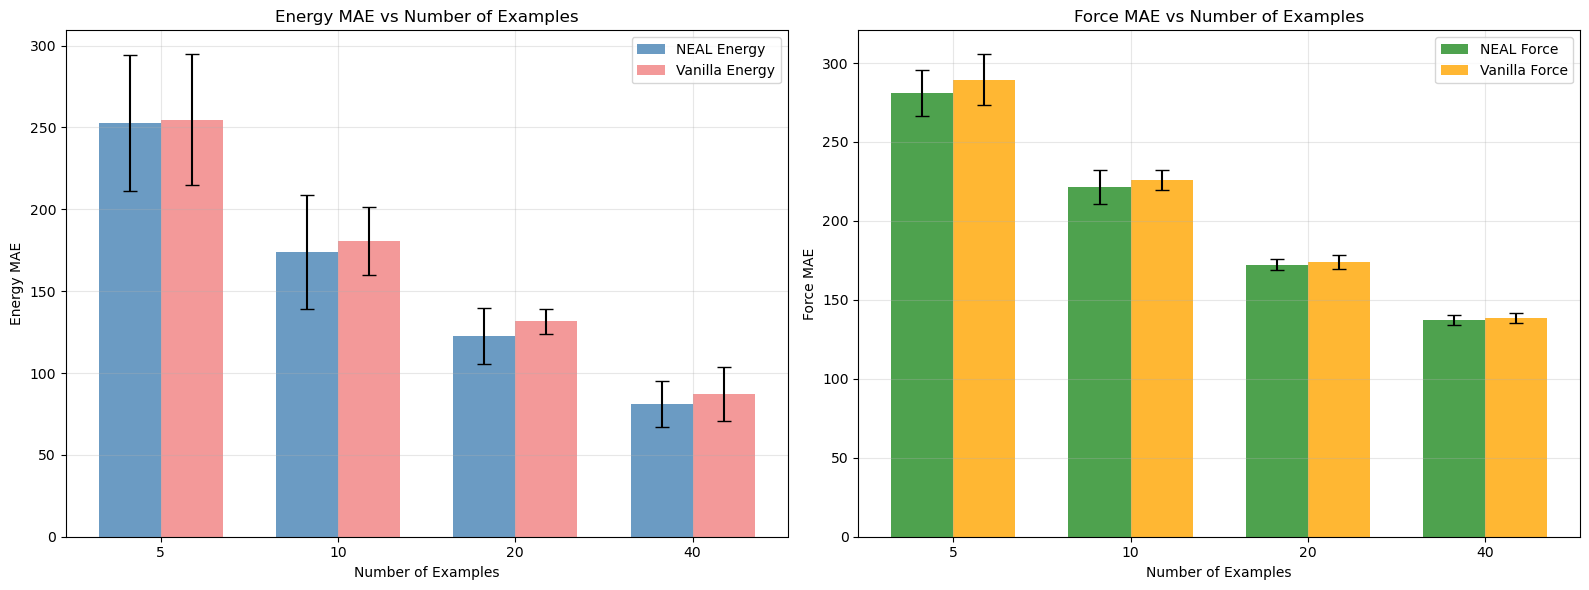
\includegraphics[width=1\linewidth]{plots/Validation using 500 examples using force mae only .png}
    \caption{Using force mae of 500 examples}
    \label{fig:placeholder}
\end{figure}

\section{Ensemble Selection Problem}
The main problem of quantifying the performance on a problem can be broken in two steps
\begin{enumerate}
    \item Identify the performance of each of the 5 models in ensemble using it's cross-validation set which it has not seen in training. 
    \item Evaluating a model on it's cross-validation set gives \textbf{2 scalars} \textbf{energy\_mae} and \textbf{force\_mae}. 
\item We aim to find the optimal scalars $\mathbf{\lambda_e}$ and $\mathbf{\lambda_f}$ such that their weighted combination
\begin{equation}
    \mathbf{\lambda_e \cdot E_{\text{mae}} + \lambda_f \cdot F_{\text{mae} }}
\end{equation}
provides the best estimate of overall model performance.
\item We will get one value for each model and the goal is to combine them. Here we have multiple choices like median, mean+std, mean-std, mean/std etc.
\end{enumerate}
\newpage
\section{Spearman Correlation}
Calculation of Spearman Correlation for a complete strategy eg ($\lambda_e=1$ $\lambda_f=0$ , median for aggregation for a fixed budget num\_eg = 10 )
\begin{enumerate}
    \item For each ensemble evaluate it on a validation set of 500 examples and \textbf{use energy mae} as the \textbf{true estimate} of the performance.
    \item \textbf{Note} that as we are focusing of energy the true estimate will never change. That is for whatever values of $\lambda_e$ and $\lambda_f$ our target remains same.
    \item For each ensemble estimate it's performance using spearman correlation.
    \item Calculate spearman correlation coefficient using these two values.
    \item \textbf{Note that we do not treat different random seeds differently.}
\end{enumerate}
\begin{figure}[htbp]
    \centering
    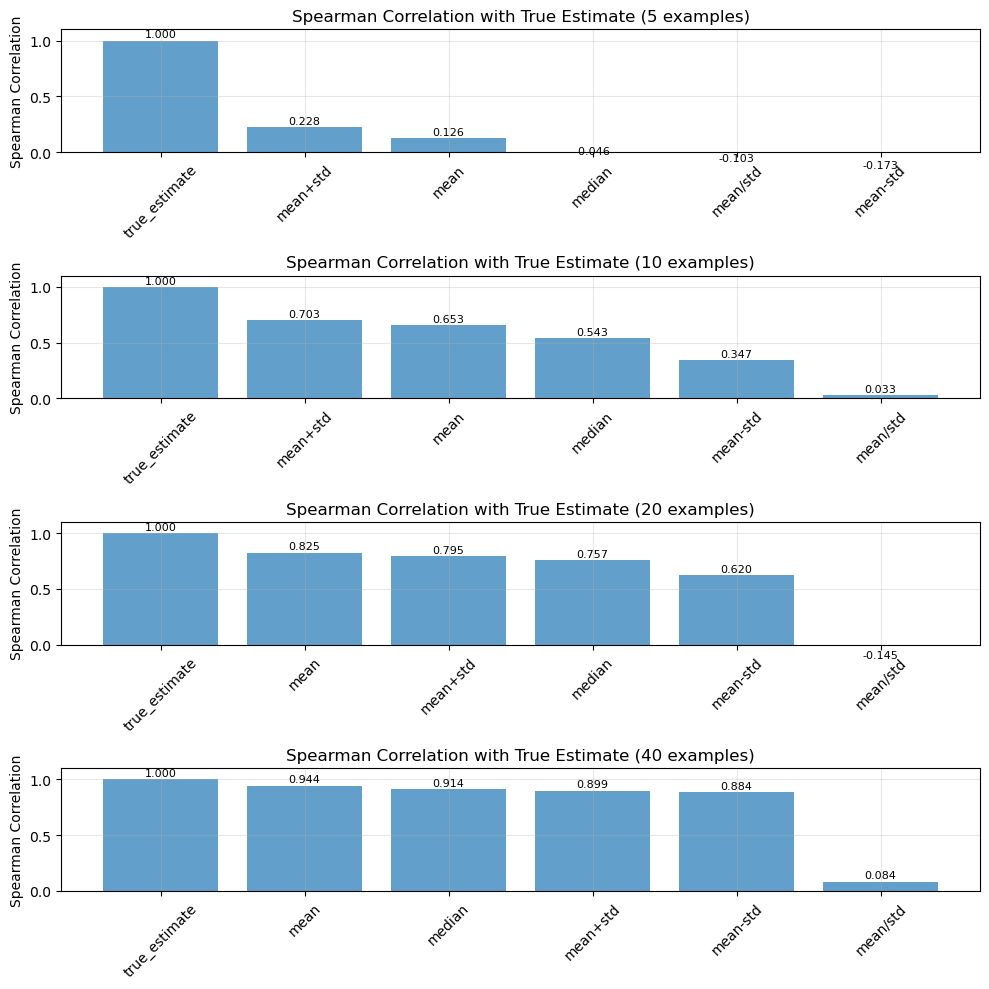
\includegraphics[width=0.75\linewidth]{plots/spearman coorelation using energy.png}
    \caption{Spearman Correlation using Energy only }
    \label{fig:placeholder}
\end{figure}
\newpage
\begin{figure}[htbp]
    \centering
    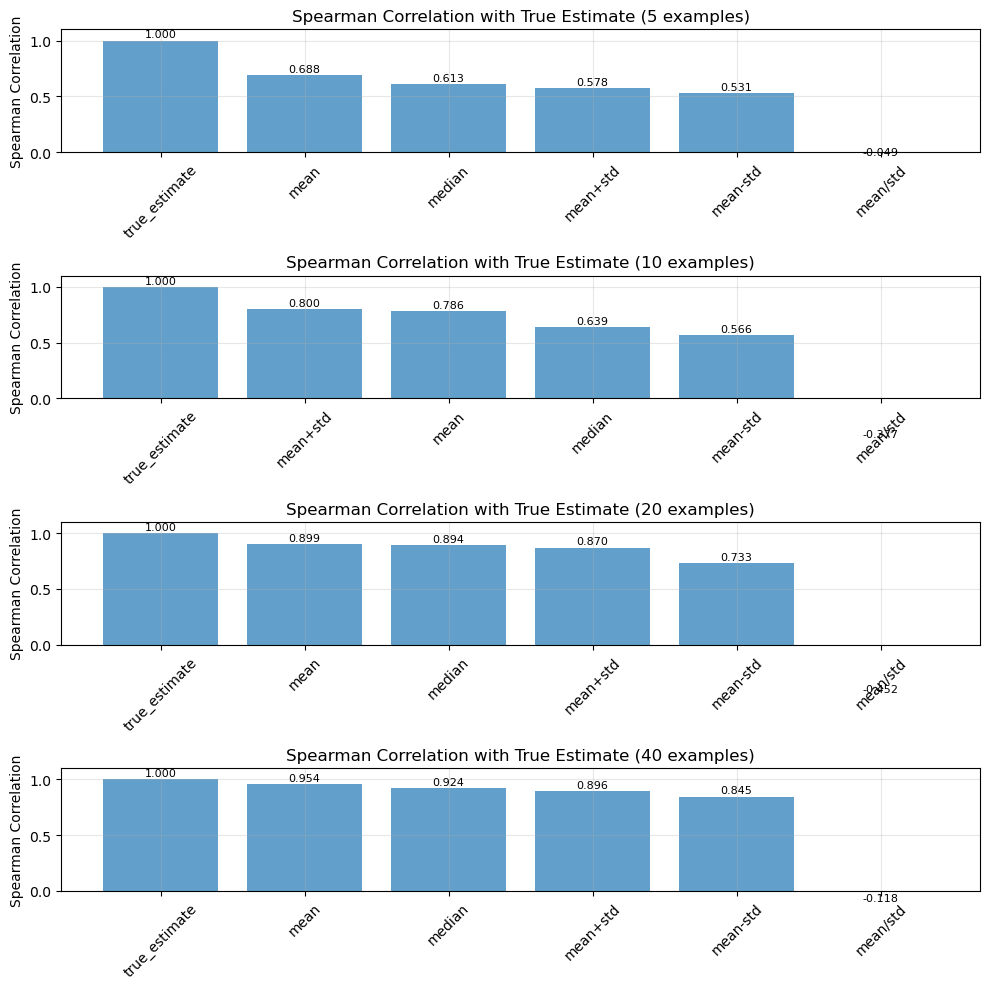
\includegraphics[width=0.75\linewidth]{plots/Spearman coreelation using force + energy use all seeds.png}
    \caption{Spearman correlation using energy mae + force mae.}
    \label{fig:placeholder}
\end{figure}
We observe that \textbf{mean} is generally the best and force + energy has higher correlation.
\begin{table}[htbp]
\centering
\small
\caption{Energy and Force MAE (mean $\pm$ std) force plus energy used for model selection .}
\begin{tabular}{@{}lcccc@{}}
\hline
\textbf{num\_ex} & \textbf{NEAL Energy MAE} & \textbf{Vanilla Energy MAE} & \textbf{NEAL Force MAE} & \textbf{Vanilla Force MAE} \\
\hline
5  & 263.19 $\pm$ 35.52 & \textbf{254.81 $\pm$ 39.76} & 294.66 $\pm$ 19.63 & \textbf{289.37 $\pm$ 16.08} \\
10 & \textbf{174.07 $\pm$ 26.55} & 180.64 $\pm$ 20.52 & \textbf{223.58 $\pm$ 9.99} & 225.99 $\pm$ 6.40 \\
20 & \textbf{111.29 $\pm$ 18.47} & 131.59 $\pm$ 7.77  & 178.66 $\pm$ 7.00  & \textbf{173.97 $\pm$ 4.24} \\
40 & \textbf{72.71 $\pm$ 5.87}   & 87.27 $\pm$ 16.59  & 138.86 $\pm$ 3.27  & \textbf{138.52 $\pm$ 2.94} \\
50 & \textbf{64.62 $\pm$ 5.16} & 77.38 $\pm$ 3.64     & \textbf{124.11 $\pm$ 3.79} & 124.61 $\pm$ 3.93
\\
\hline
\end{tabular}
\end{table}

\newpage
\section{Using method suggested by Rushikesh}
Method: For each budget,strategy and seed calculate spearman correlation. Then avg across seeds to get the result for a strategy at this budget.

\begin{figure}[htbp]
    \centering
    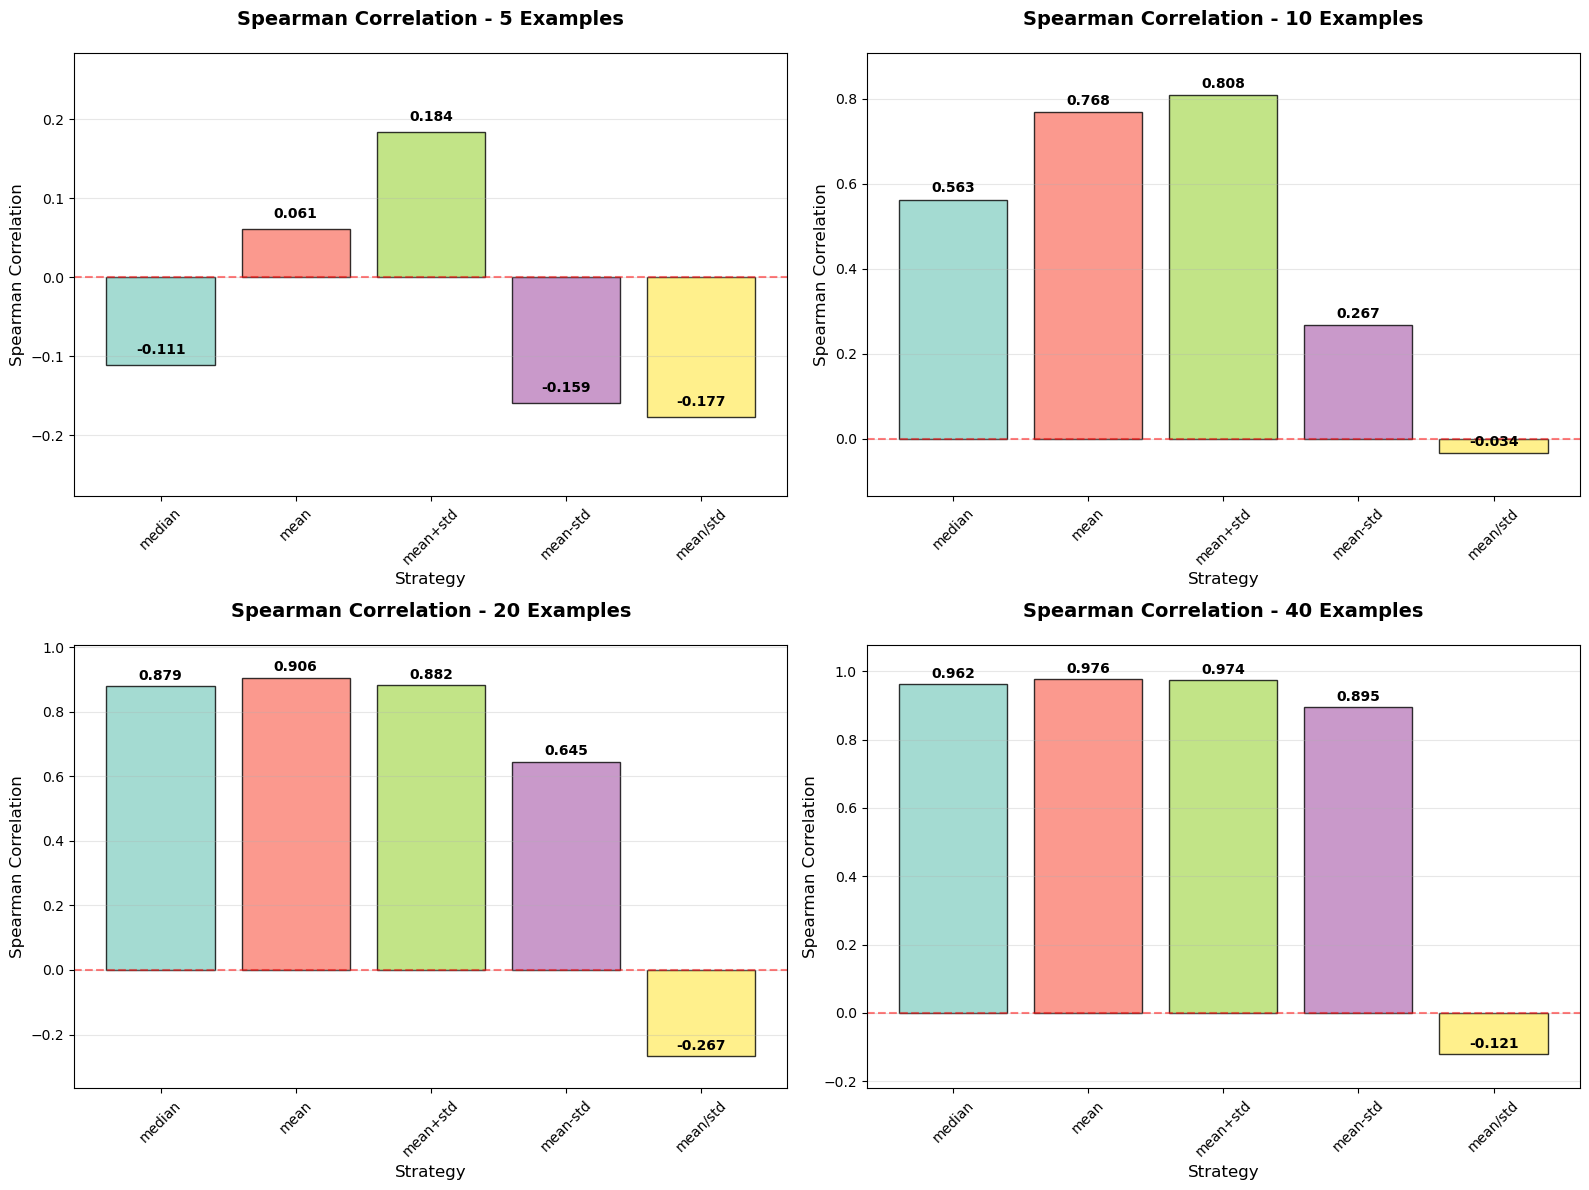
\includegraphics[width=0.75\linewidth]{plots/spearman correlation avg.png}
    \caption{Spearman Correlation using energy mae for different strategies averaged across seeds.}
    \label{fig:placeholder}
\end{figure}
\newpage
\begin{figure}[htbp]
    \centering
    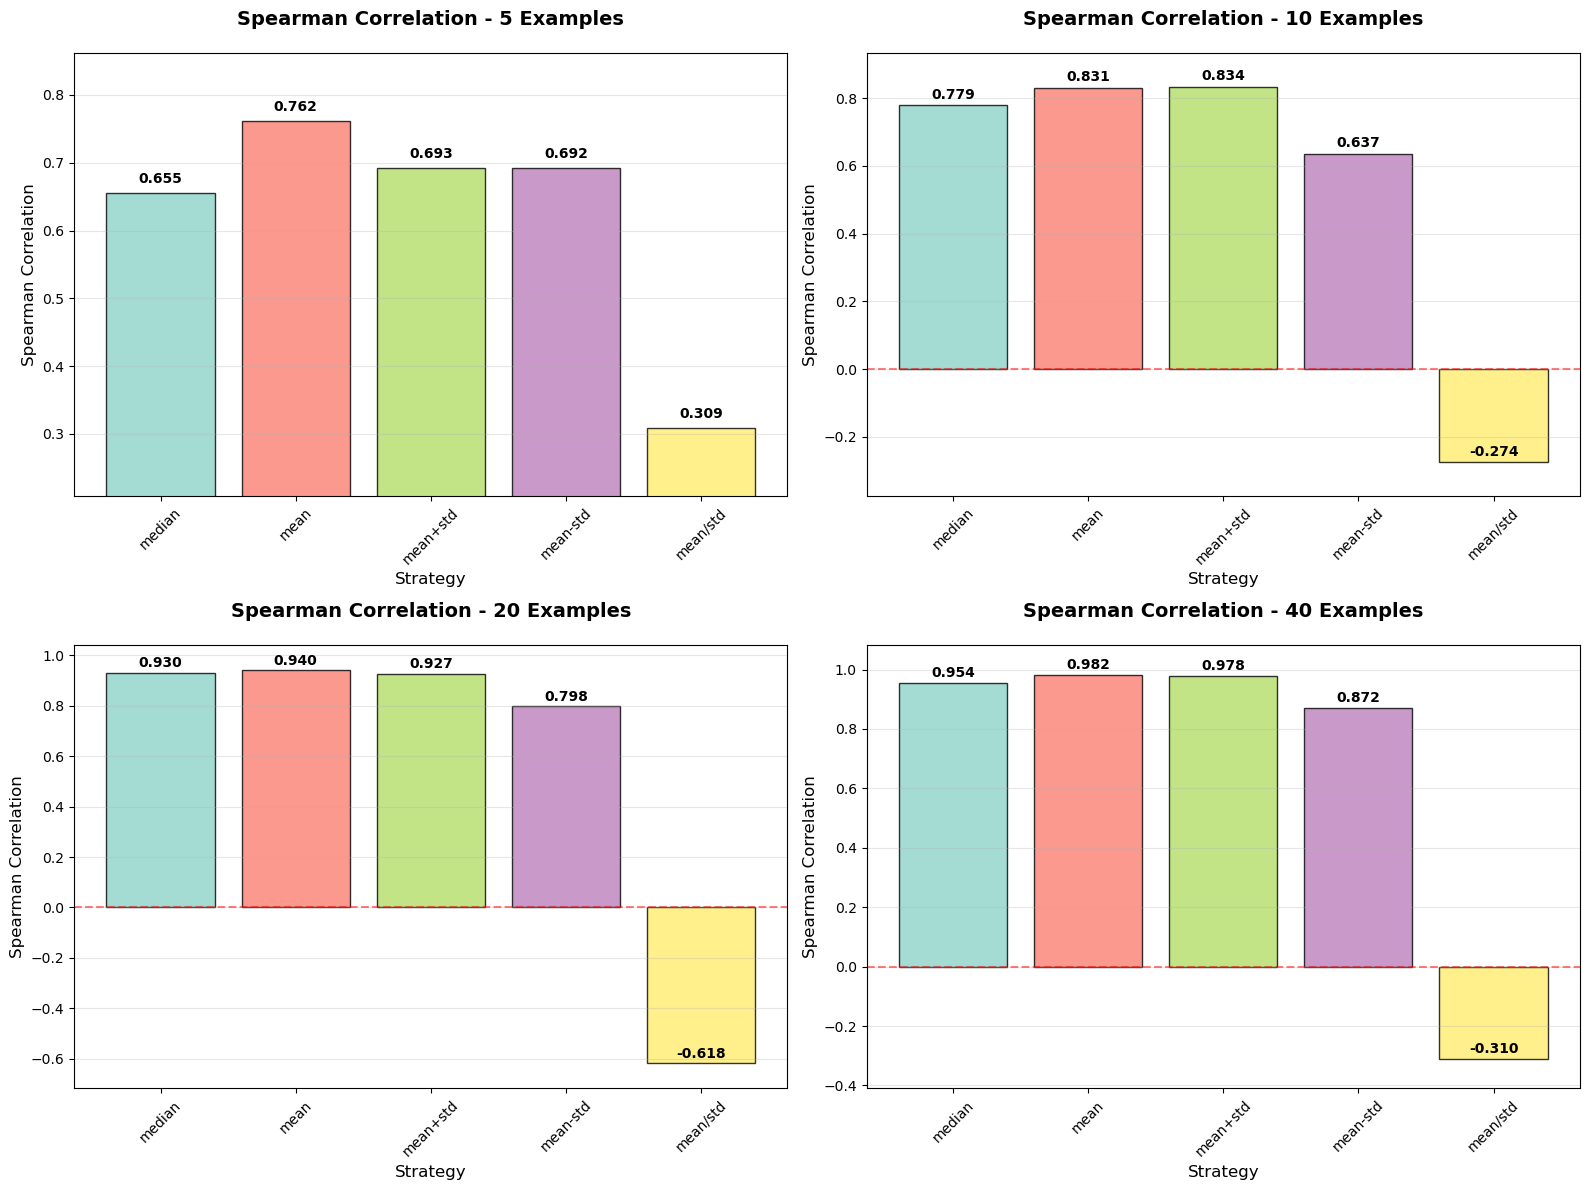
\includegraphics[width=0.75\linewidth]{plots/spearman correlation using energy mae + force mae averaged across 5 seeds.png}
    \caption{Spearman correlation using energy and force averaged across 5 seeds.}
    \label{fig:placeholder}
\end{figure}



    
\end{document}